\chapter{Planteamiento del problema y primer acercamiento} \label{cap1}

En este capítulo se presenta el dilema general del trabajo, el hardware sobre el que se
experimenta y el primer acercamiento al objetivo: la integración de GPUs de distinta naturaleza
en un mismo sistema.

\section{La limitación del driver único}

El punto de partida del trabajo es una restricción técnica fundamental: \textbf{en un mismo 
sistema operativo no puede haber más de una versión de driver propietario cargada al mismo tiempo}. 
El motivo es que el módulo del driver (\texttt{nvidia.ko}) controla elementos globales del 
\textit{kernel}, no solo de cada tarjeta individual: gestiona la memoria unificada, registra 
los archivos de comunicación con el sistema (\texttt{character devices}) y expone funciones globales 
en el núcleo. Cargar dos versiones distintas sobre el mismo sistema generaría un conflicto directo 
por el control de estos recursos. Esta limitación es ampliamente conocida en sistemas de esta índole
y es precisamente la línea conductora que define todas las decisiones tomadas a lo largo de este proyecto.

Partiendo de esta premisa, surgen dos escenarios posibles:
\begin{enumerate}
    \item \textbf{Un único driver para todas las GPUs:} Es viable únicamente si todas las tarjetas 
    instaladas comparten una misma versión de driver. Esto limita bastante el hardware 
    que se puede combinar en una misma máquina, ya que exige utilizar tarjetas de épocas similares que compartan 
    soporte. 
    Este es precisamente nuestro caso de estudio: se dispone de dos Tesla C1060 y una ASUS ENGTS 250, modelos compatibles con la misma rama de drivers \textit{legacy} de NVIDIA. La configuración experimental empleó una Tesla C1060 y la ENGTS250, porque la tercera tarjeta no fue detectada a través del \textit{riser} PCIe.
    \item \textbf{Aislamiento de cada tarjeta en un entorno propio:} Cada GPU se asigna de forma 
    exclusiva a una máquina virtual con su propio sistema operativo y su propia versión de driver. 
    Esta vía evita por completo la limitación del driver único, a cambio de la complejidad técnica 
    que supone configurar el paso directo (\textit{passthrough}) con VFIO.
\end{enumerate}

Es digno de mención que el uso de contenedores (como Docker o LXC) no resuelve este problema: 
los contenedores aíslan aplicaciones y librerías en el espacio de usuario, pero todos comparten 
obligatoriamente el mismo \textit{kernel} y el mismo módulo de driver cargado en el anfitrión. 
Esta diferencia entre aislar procesos por software y aislar hardware real es una de las piedras
angulares de este trabajo.

\section{Descripción del entorno hardware}

El entorno sobre el que se ha desarrollado todo el trabajo es el siguiente:

\begin{table}[htbp]
\centering
\begin{tabular}{|l|l|}
\hline
\textbf{Componente} & \textbf{Valor} \\
\hline
Placa base & ASUS TUF GAMING X670E-PLUS WIFI                             (con iGPU integrada)\\
\hline
CPU & AMD Ryzen 9 7950X 16-Core Processor\\
\hline
Hipervisor & Proxmox VE 9.2.0 \\
\hline
GPU 1 & NVIDIA Tesla C1060 (GT200, cómputo) \\
\hline
GPU 2 & ASUS ENGTS250 (GT200, consumo) \\
\hline
Driver objetivo & NVIDIA 340.108 \\
\hline
\end{tabular}
\caption{Entorno hardware del trabajo}
\label{tab:entorno}
\end{table}

El detalle de las especificaciones de las GPUs se presentó en la tabla \ref{tab:gpus} del capítulo de preliminares. Tanto la placa base como la CPU son componentes modernos (2022--2025), lo cual, como veremos, introduce problemas de compatibilidad con los sistemas operativos antiguos que el hardware \textit{legacy} requiere.

\subsection{Configuración de firmware de la plataforma}

En este apartado se detallan los parámetros modificados en el firmware de la placa base 
con el fin de acondicionar el arranque del sistema a las restricciones operativas de un 
hardware gráfico tan antiguo como el que se emplea en este trabajo.

Como primer objetivo, estaba lograr que la plataforma superase con éxito la fase 
de inicialización POST (\textit{Power-On Self-Test}), etapa de autodiagnóstico en la que el 
firmware escanea, asigna recursos y enumera los dispositivos conectados a los buses antes de 
transferir el control al cargador de arranque.

Dada la arquitectura de las tarjetas empleadas (familia GT200 y derivadas), resulta imprescindible 
habilitar el módulo de compatibilidad CSM (\textit{Compatibility Support Module}) con prioridad de 
ejecución para memorias \textit{Legacy OpROM}. La \textit{OpROM} es la memoria no volátil en la que reside 
la VBIOS (\textit{Video BIOS}) de la GPU,
el código mínimo
ejecutable requerido para que la placa base pueda comprobarla y dar paso al arranque del sistema
operativo. Dada la generación a la que se remonta el hardware legacy de este trabajo, su VBIOS carece
del protocolo moderno GOP (\textit{Graphics Output Protocol}), 
estándar requerido por las plataformas UEFI para inicializar la salida de vídeo durante el POST. 

Como consecuencia directa, un arranque configurado en modo UEFI nativo puro provoca un bloqueo temprano en el POST: 
la placa base es incapaz de ejecutar el controlador de la memoria ROM de la GPU para inicializar el dispositivo 
antes de ceder el control al sistema operativo. La activación del módulo CSM solventa esta incompatibilidad 
emulando un entorno BIOS tradicional, lo que permite ejecutar el código de 16 bits de la VBIOS y completar 
la secuencia de inicialización del bus PCIe.

En segundo lugar, dado que este es un sistema multi-GPU, es necesario configurar también la distribución eléctrica de 
las líneas de datos (\textit{lanes}) para evitar que el 
firmware asigne la totalidad del ancho de banda al bus principal, manteniendo operativas ambas ranuras, principal y
secundaria de forma concurrente.

Durante las pruebas se forzó manualmente el enlace de las ranuras a PCIe Gen~1. Si bien esto supone una 
pérdida considerable de ancho de banda, asegura una comunicación más tolerante y evita que el bus actual 
descarte las tarjetas antiguas ante discrepancias en los tiempos de respuesta.

\subsection{Arranque dual LXC/VFIO} \label{sec:arranque}

Las configuraciones de LXC y VFIO no pueden convivir en el mismo arranque: la primera necesita que el anfitrión cargue el driver NVIDIA, mientras que la segunda necesita reservar las GPUs para \texttt{vfio-pci}. Por ello se implantó un arranque dual mediante GRUB, el gestor que presenta el menú inicial del sistema y selecciona el kernel y sus parámetros.

El arranque por defecto corresponde al modo LXC, por ser la configuración más estable. Para los experimentos con máquinas virtuales se añadió una entrada personalizada de GRUB que arranca el mismo kernel con parámetros orientados a VFIO:

\begin{lstlisting}[style=bash]
pcie_port_pm=off pcie_aspm=off amd_iommu=on iommu=pt pci=noaer \
  vfio_pci.disable_idle_d3=1 vfio_pci.disable_vga=1 vfio_dynamic
\end{lstlisting}

Además, los módulos \texttt{vfio}, \texttt{vfio\_iommu\_type1}, \texttt{vfio\_pci} y \texttt{vfio\_virqfd} quedan disponibles para que el hardware pueda vincularse a \texttt{vfio-pci}. La palabra \texttt{vfio\_dynamic} no es una opción estándar del kernel: es una marca local introducida expresamente para identificar este arranque.

La selección de VFIO es de un solo arranque. El comando \texttt{boot-vfio} fija dicha entrada únicamente para el próximo reinicio y cancela la operación si GRUB no acepta la selección; \texttt{GRUB\_DEFAULT} permanece en la entrada estable de LXC. Un servicio \textit{one-shot} limpia después la variable interna \texttt{next\_entry}, de modo que los reinicios siguientes vuelven automáticamente al modo LXC. El comando \texttt{check-mode} inspecciona \texttt{/proc/cmdline} y muestra las GPUs detectadas con su driver activo.

Con esta base común de plataforma ya estabilizada, el primer experimento consistió en probar la vía más directa: un sistema Ubuntu con soporte nativo para el driver antiguo.

\section{Primer acercamiento: Ubuntu 18.04 LTS con el driver 340.40}

La primera aproximación al problema consistió en instalar un sistema operativo relativamente 
antiguo ---Ubuntu 18.04 LTS (núcleo 4.15, GCC 7.x)--- por contar con soporte directo para el 
controlador requerido por las tarjetas. En esta versión, el paquete \texttt{nvidia-340} de los 
repositorios oficiales de Canonical se instalaba sin fricción, ya que la distribución mantenía 
binarios y parches preparados específicamente para dicho \textit{kernel}.

La instalación resultó sencilla y el controlador detectó ambas GPUs sin inconvenientes. Sin embargo, 
este acercamiento pronto mostró sus limitaciones. Tanto la placa base como el procesador del equipo 
de pruebas son componentes posteriores a esta versión de Ubuntu, por lo que un \textit{kernel}
anterior carece del soporte adecuado para la gestión del \textit{chipset} moderno. 

A esto se sumó el aspecto verdaderamente crítico para los objetivos del trabajo: Ubuntu 18.04, 
con su \textit{kernel} base 4.15, no permitía un particionamiento limpio de los grupos IOMMU ni 
ofrecía una pila de virtualización suficientemente actualizada para gestionar los dispositivos 
PCIe con garantías. Al no reconocer la topología de interconexión de la placa base moderna, el 
\textit{kernel} antiguo agrupaba múltiples periféricos independientes dentro de un mismo grupo IOMMU por 
motivos de seguridad de memoria. Dado que el paso directo mediante VFIO exige aislar el grupo al 
completo, resultaba inviable desacoplar una única tarjeta sin arrastrar otros componentes del sistema.

Por otro lado, actualizar dicho núcleo a una versión más reciente para solventar este problema 
rompía de inmediato el módulo \texttt{nvidia-340}, cuyo código fuente no estaba adaptado a las 
interfaces internas de memoria de los \textit{kernels} posteriores. Ante este conflicto, mantener 
el sistema anfitrión en esta distribución impedía disponer simultáneamente del soporte moderno 
para aislar los dispositivos por hardware y del entorno necesario para operar las tarjetas.

\section{Marco de decisión: ¿cuándo compensa este sistema?} \label{sec:marco_decision}

Con los fundamentos de la sección~\ref{sec:fundamentos} (leyes de Amdahl/Gustafson, Roofline y modelo PCIe/coste), se aplica aquí el marco introducido en los preliminares. La figura~\ref{fig:arbol_viabilidad} resume los cinco filtros; basta con que uno falle para que el despliegue no compense y deba descartarse o replantearse. Este capítulo concreta dicho marco para el caso de estudio.

\begin{figure}[htbp]
\centering
% Figura precompilada para reducir el tiempo de compilacion.
% Fuente editable: figuras/capitulo1/arbol-viabilidad.tex
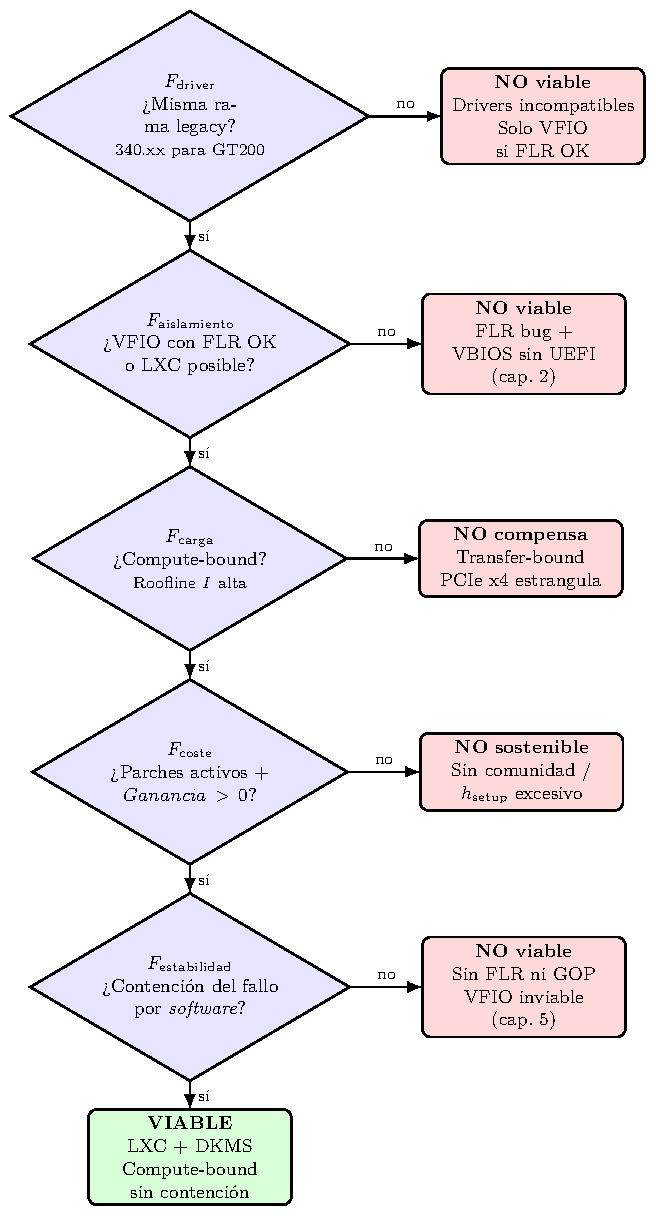
\includegraphics[height=0.60\textheight,keepaspectratio]{figuras/capitulo1/arbol-viabilidad}
\caption{\'Arbol de decisi\'on de viabilidad $V = F_{\text{driver}} \land F_{\text{aislamiento}} \land F_{\text{carga}} \land F_{\text{coste}} \land F_{\text{estabilidad}}$ aplicado al caso de estudio. Los cap\'itulos 2--5 recorren cada filtro en orden; $F_{\text{estabilidad}}$ se particulariza en la secci\'on~\ref{sec:marco_viabilidad} de los preliminares.}
\label{fig:arbol_viabilidad}
\end{figure}

\textbf{F1. Homogeneidad de driver} \cite{nvidia_legacy_driver,nvidia_legacy_support}. ¿Comparten todas las GPUs la misma rama legacy? En nuestro caso sí \cite{michelboucey}: GT200 $\to$ 340.108. Si no, la vía LXC queda bloqueada por la limitación del driver único descrita en este capítulo \cite{nvidia_forum_multidriver}; solo queda VFIO, que exige pasar al siguiente filtro.

\textbf{F2. Aislamiento} \cite{kernel_vfio,proxmox_pci_passthrough,supermicro_gpu_passthrough}. ¿La plataforma permite aislar cada GPU? Requiere IOMMU activa, grupo IOMMU dedicado \cite{heiko_iommu_groups} y FLR correcto \cite{pcisig2022,amd_pg344_flr}. Nuestro hardware falla en FLR (capítulo~2): VFIO inviable, pero LXC sí lo es porque comparte el driver del host y no necesita reset. Si ambos fallan, no hay vía.

\textbf{F3. Perfil de carga} \cite{williams2009roofline,amdahl1967}. ¿La aplicación es \textit{compute-bound}? Evaluar con Roofline: si $T_{\text{compute}} \gg B/BW_{\text{PCIe}}$ (ecuación de la sección~\ref{sec:roofline}), las lanes no importan. En el capítulo~\ref{cap5} demostramos que \texttt{matrixMul} lo es (sin contención con 2 GPUs concurrentes), por lo que el estrangulamiento PCIe del slot chipset no penaliza. Si la carga es \textit{transfer-bound}, la plataforma de consumo con x4 vía chipset \cite{asusx670e,amd7950x} hace que no compense frente a servidor con 64--128 lanes directas \cite{pcisig2022}.

\textbf{F4. Coste y sostenibilidad} \cite{michelboucey,archlinuxjerry}. ¿Existe mantenimiento comunitario y la ganancia supera el coste? Formalmente $Ganancia = S_{\text{real}}\cdot V_{\text{hora}} - (C_{\text{kWh}}\cdot h + C_{\text{ing}}\cdot h_{\text{setup}}) > 0$. El capítulo~3 cuantifica $h_{\text{setup}}$: 7 años de drift, 21 parches, toolchain gcc. Sin los repositorios comunitarios, $C_{\text{riesgo}}\to\infty$. Este es el filtro que convierte un éxito técnico puntual en un despliegue sostenible.

\textbf{F5. Estabilidad y contención del fallo} \cite{amd_pg344_flr,uefi_gop_amd}. ¿Existe algún mecanismo por \textit{software} capaz de recuperar una GPU colgada? Requiere, en el caso de VFIO, que el FLR funcione \cite{pcisig2022,amd_pg344_flr} y que la tarjeta disponga de GOP para el handover a la VM \cite{uefi_gop_amd}. En nuestro caso fallan ambos (capítulo~2), por lo que $F_{\text{estabilidad}}=\text{falso}$ y el despliegue se descarta como tal, tal y como se formaliza en la sección~\ref{sec:marco_viabilidad} de los preliminares.

La utilidad del marco es que anticipa el resultado sin necesidad de ejecutar: nuestro caso pasa F1--F4 pero falla F5 en la vía VFIO y solo se resuelve con LXC, que no requiere aislamiento; un caso con una Kepler (driver 470) + GT200 (340) fallaría ya en F1, y una carga de streaming fallaría en F3.

